\begin{frame}{A simple example: iris data}

We fit a Gaussian mixture model with a Bayesian non-parametric prior to
the iris data.

\begin{figure}[!h]
  \centering
  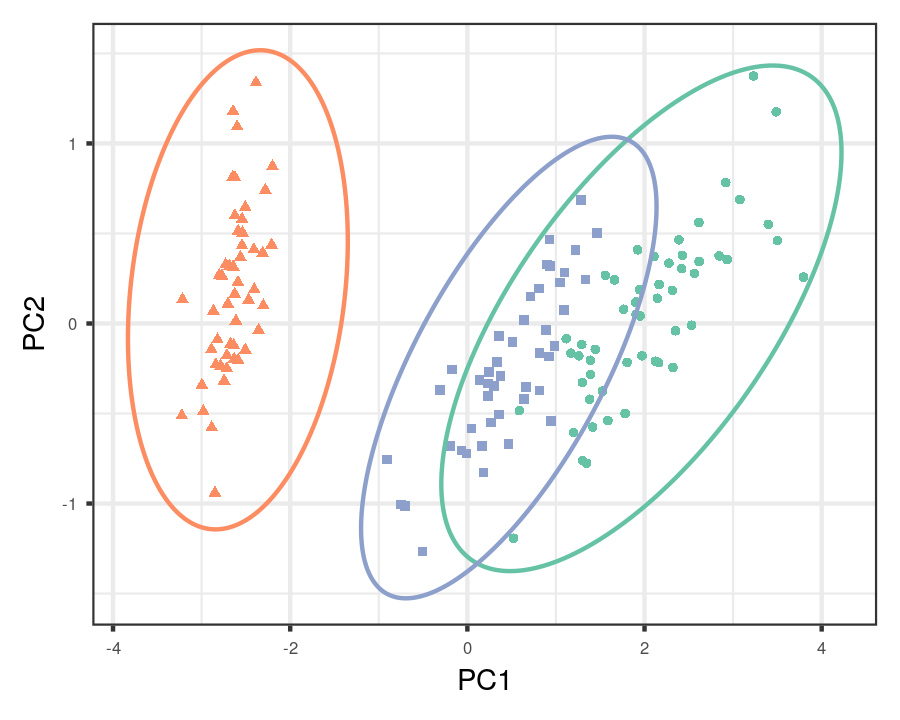
\includegraphics[width = 0.6\textwidth]{./figures/iris_init_fit.png}
  \caption*{The iris data in principal component space and GMM fit at $\alpha = 6$.}
\end{figure}

\end{frame}

\begin{frame}{iris data: parametric sensitivity}
  \begin{figure}[!h]
    \centering
    \only<1>{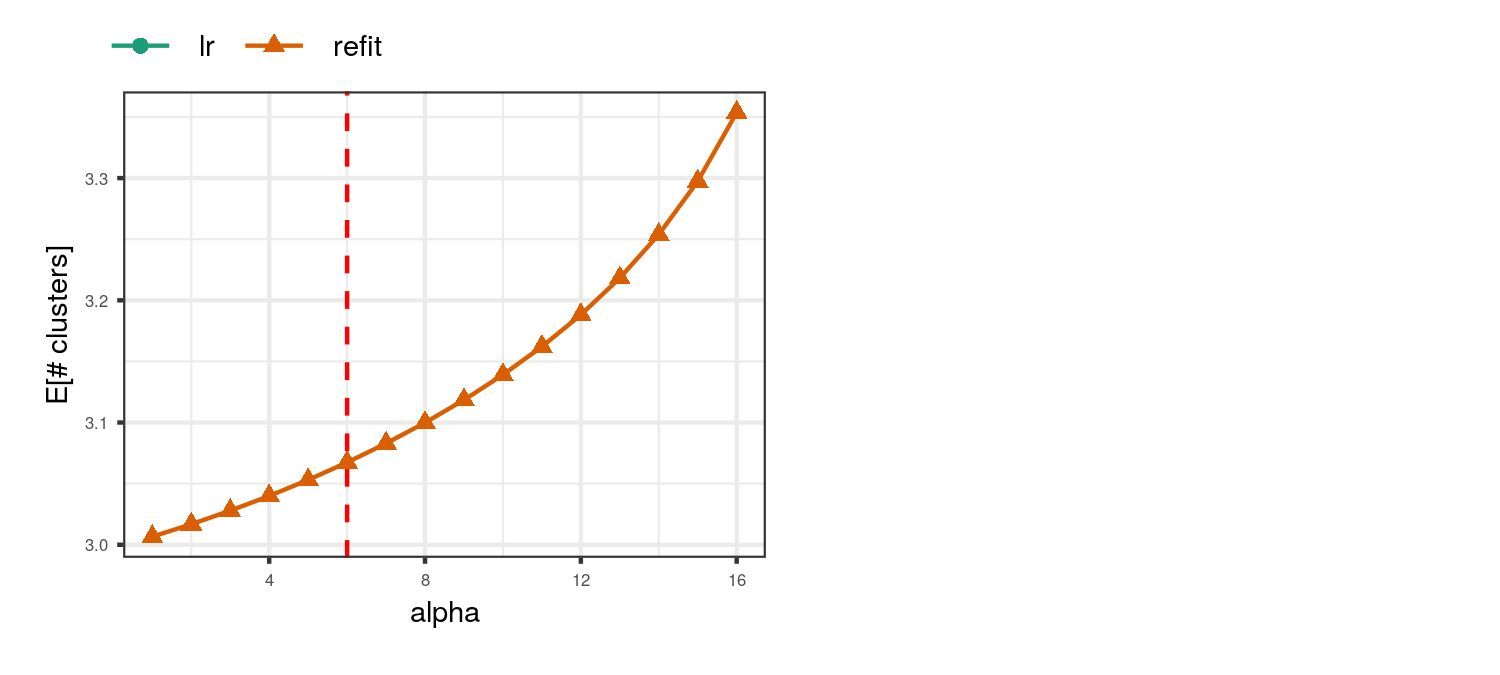
\includegraphics[width = \textwidth]{./figures/iris_alpha_sens0.png}}
    \only<2>{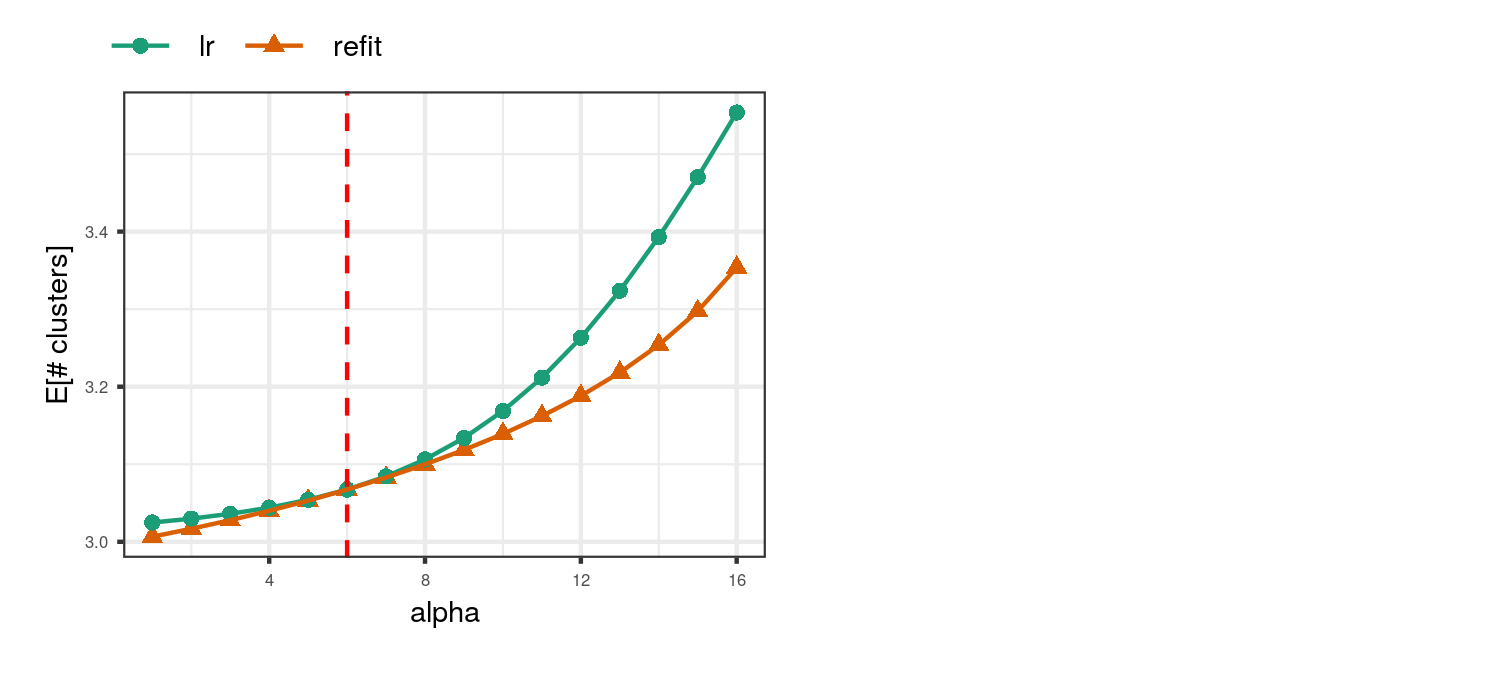
\includegraphics[width = \textwidth]{./figures/iris_alpha_sens1.png}}
    \only<3>{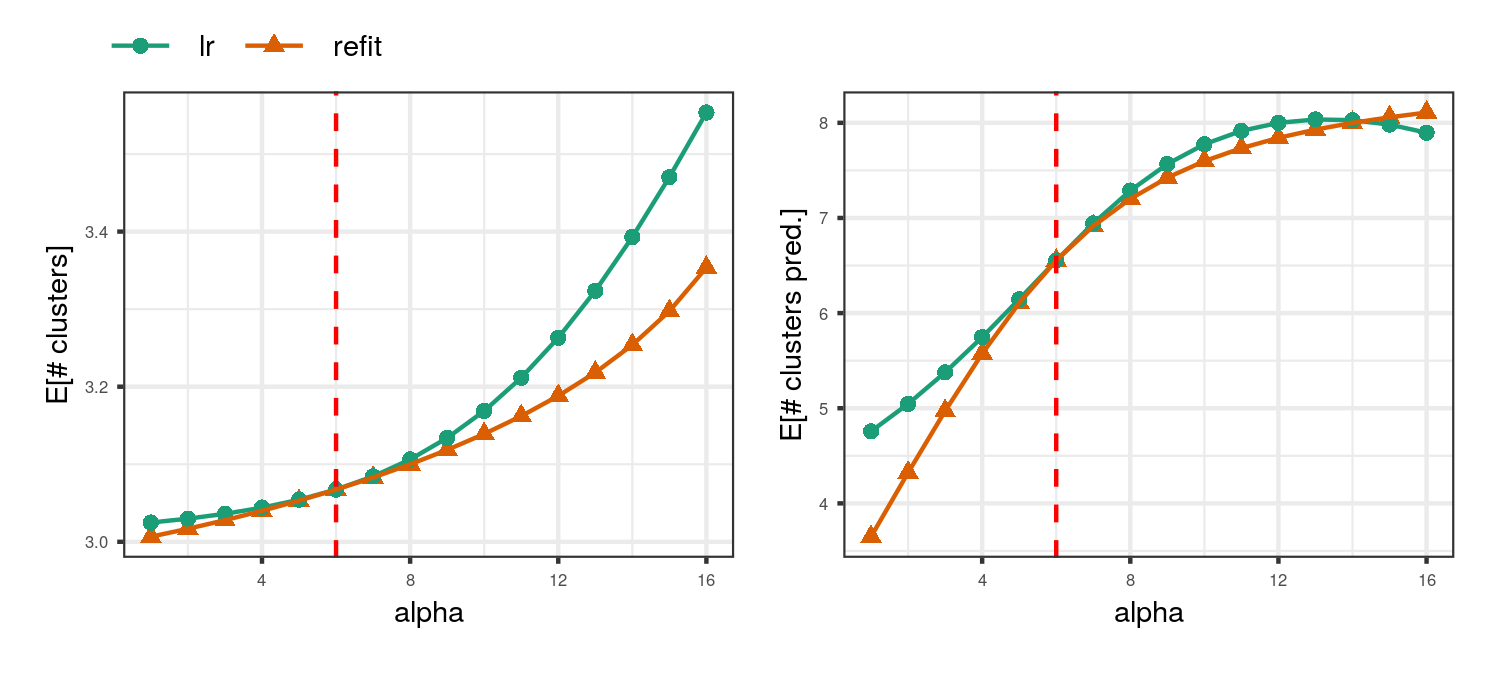
\includegraphics[width = \textwidth]{./figures/iris_alpha_sens2.png}}
    \caption*{The expected number of posterior clusters in the iris data as $\alpha$ varies.}
  \end{figure}

\end{frame}

\begin{frame}{iris data: influence functions}
  \begin{figure}[!h]
    \centering
    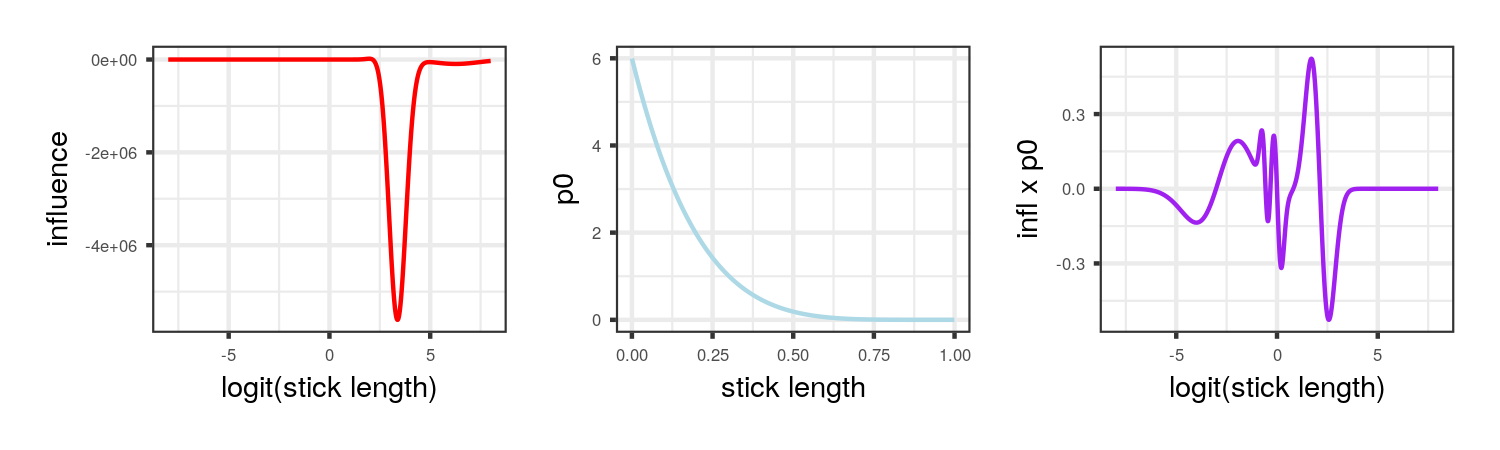
\includegraphics[width = \textwidth]{./figures/iris_influence_function.png}
    \caption*{The influence function of the expected number of predicted clusters.}
\end{figure}
\end{frame}

\begin{frame}{iris data: functional perturbations}
  \begin{figure}[!h]
    \centering
    \only<1>{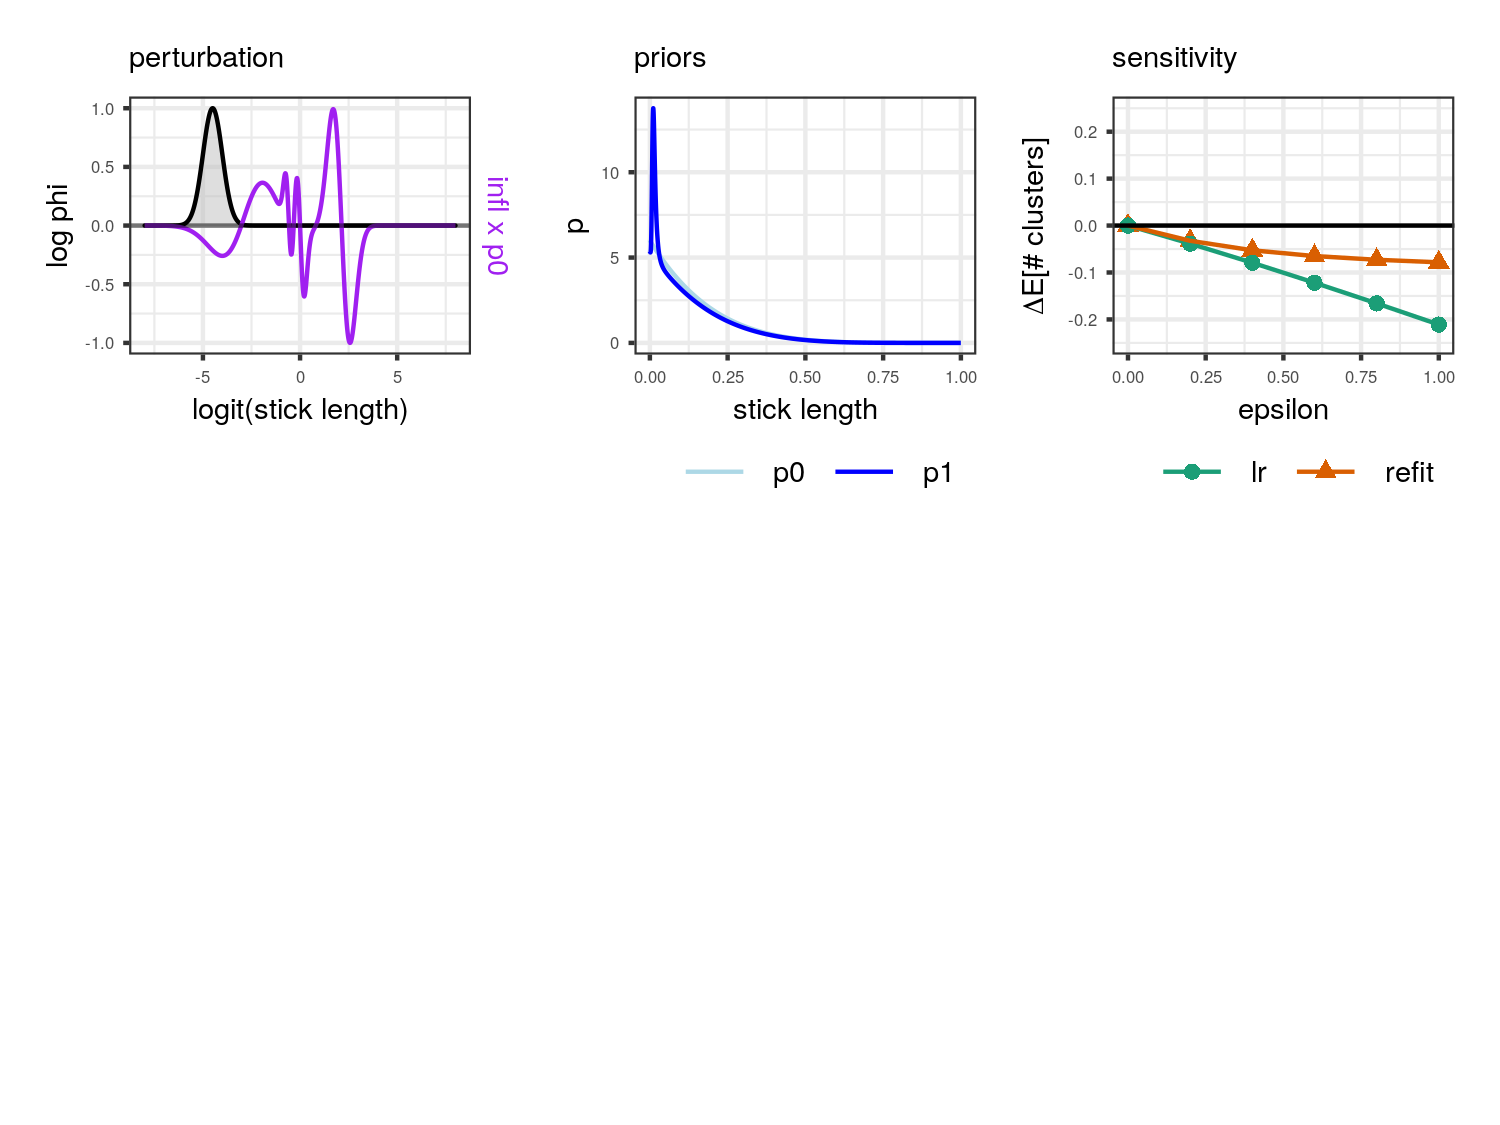
\includegraphics[width = \textwidth]{./figures/iris_func_sens0.png}}
    \only<2>{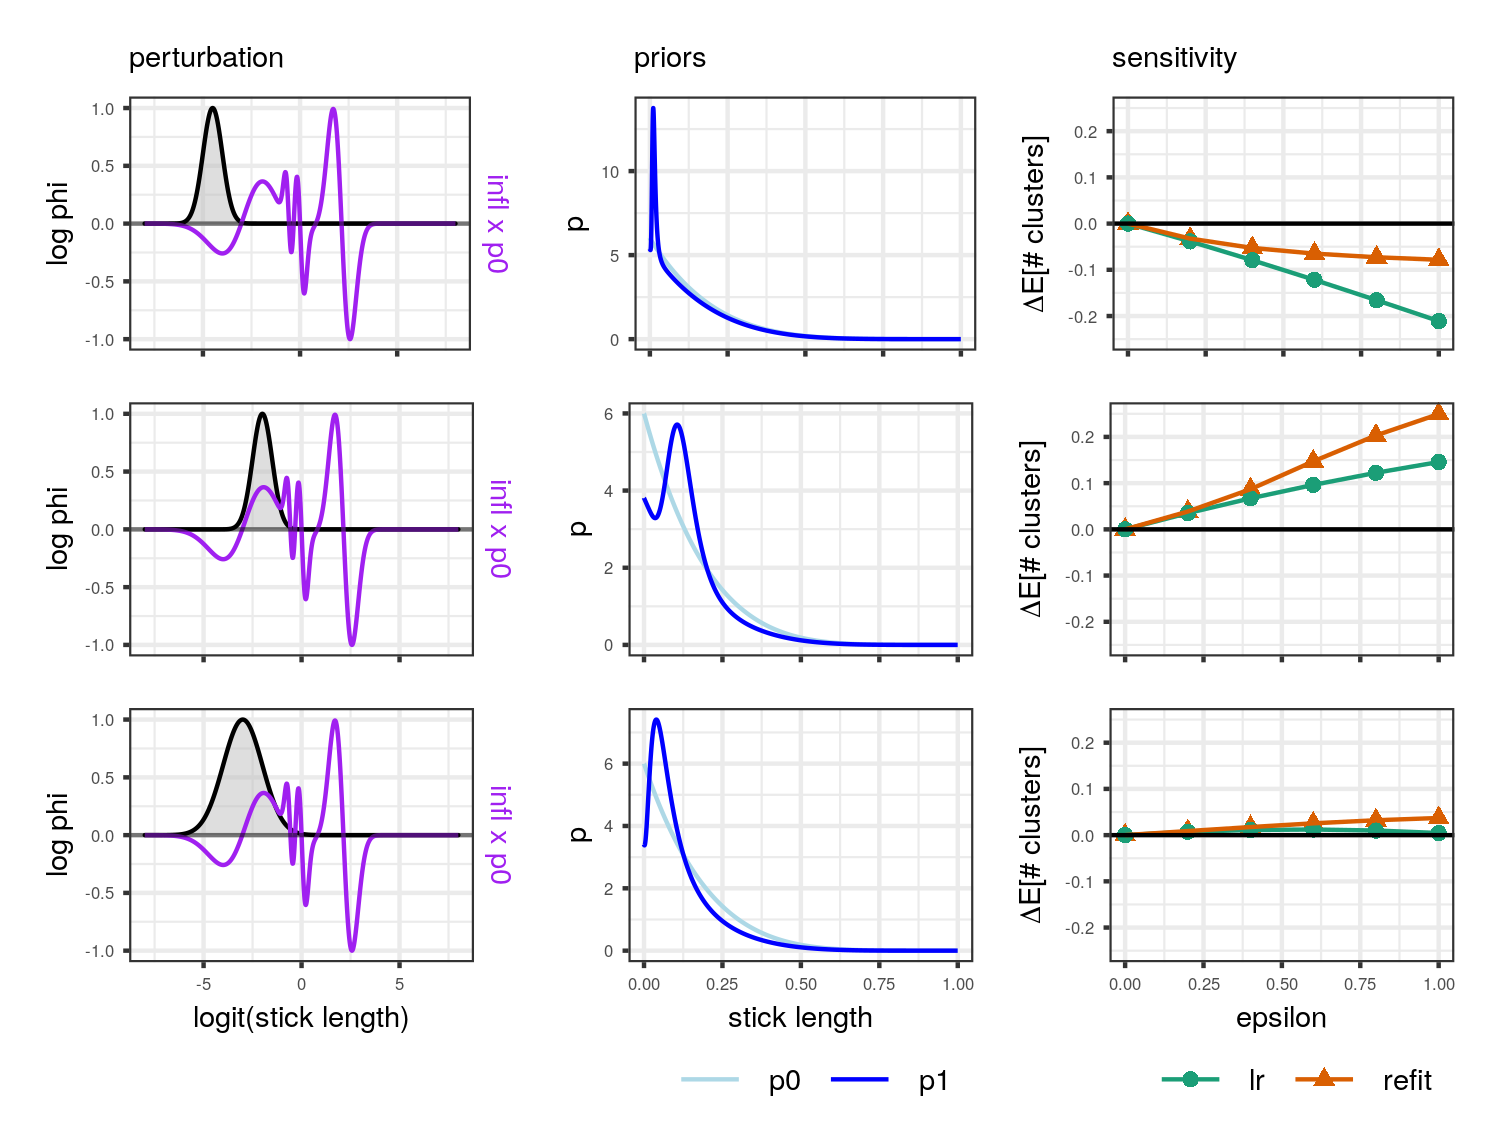
\includegraphics[width = \textwidth]{./figures/iris_func_sens1.png}}
\end{figure}
\end{frame}


\begin{frame}{iris data: worst-case perturbation}
  \begin{figure}[!h]
    \centering
    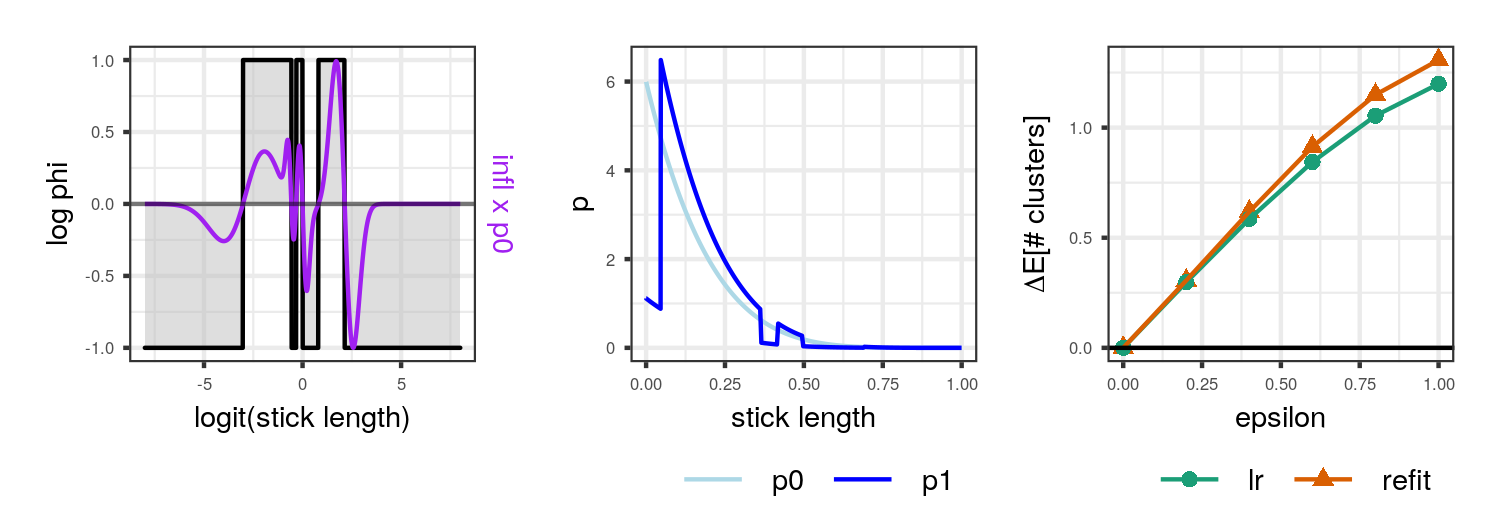
\includegraphics[width = \textwidth]{./figures/iris_worst_case.png}
\end{figure}
\end{frame}
